
\documentclass[11pt,a4paper,UTF8]{book}

\usepackage[T1]{fontenc}
\usepackage[utf8]{inputenc}
\usepackage{authblk}

\usepackage{fontspec}                  %引入字体设置宏包
\setmainfont{Times New Roman}             %设置英文正文字体
% Courier New
% Book Antique
\setsansfont{Arial}                    %英文无衬线字体
\setmonofont{Courier New}              %英文等宽字体

\usepackage{ctex} %导入中文包
%\usepackage{ulem}
\usepackage{tocvsec2}
\usepackage{verbatim}

\usepackage{tabularx}
\usepackage{booktabs} 
\usepackage{multirow}
\usepackage{bbding}
\usepackage{float}
\usepackage{xspace}
\usepackage[none]{hyphenat}

\usepackage{graphicx}
\usepackage{subfigure}
\usepackage{pifont}

\usepackage{hyperref}  %制作pdf的目录
\usepackage{subfiles} %使用多文件方式进行

\usepackage{geometry} %设置页边距的包
\geometry{left=2.5cm,right=2cm,top=2.54cm,bottom=2.54cm} %设置书籍的页边距

\usepackage{url}
\hypersetup{hidelinks, %去红框
  colorlinks=true,
  allcolors=black,
  pdfstartview=Fit,
  breaklinks=true
}

% 调整itemlist中的行间距
\usepackage{enumitem}
\setenumerate[1]{itemsep=0pt,partopsep=0pt,parsep=\parskip,topsep=5pt}
\setitemize[1]{itemsep=0pt,partopsep=0pt,parsep=\parskip,topsep=5pt}
\setdescription{itemsep=0pt,partopsep=0pt,parsep=\parskip,topsep=5pt}

% 超链接样式设置
\usepackage{hyperref}
\hypersetup{
  colorlinks=true,
  linkcolor=blue,
  filecolor=blue,
  urlcolor=blue,
  citecolor=cyan,
}

\usepackage{indentfirst}

\usepackage{listings}
\usepackage[usenames,dvipsnames,svgnames, x11names]{xcolor}

\usepackage[most]{tcolorbox}
\tcbuselibrary{breakable} % 引入 breakable 库
\tcbuselibrary{skins} % 引入 skins 库

%展示代码
\definecolor{mygreen}{rgb}{0,0.6,0}
\definecolor{mygray}{rgb}{0.5,0.5,0.5}
\definecolor{mymauve}{rgb}{0.58,0,0.82}
\definecolor{keywordcolor}{rgb}{0.8,0.1,0.5}
\definecolor{webgreen}{rgb}{0,.5,0}
\definecolor{bgcolor}{rgb}{0.92,0.92,0.92}

%定义CMake
\lstdefinelanguage{CMake}
{morekeywords={
    cmake\_minimum\_required,
    project,
    add\_executable,
    add\_library,
    target\_link\_libraries,
    cmake\_parse\_arguments,
    cmake\_language,
    set, unset,
    option,
    string,
    list,
    math,
    message,
    if, elseif, else, endif,
    mark\_as\_advanced,
    foreach, endforeach,
    while, endwhile,
    add\_subdirectory, include, return, include\_gurad,
    function, endfunction,
    macro, endmacro,
    find\_package,
    cmake\_push\_check\_state,
    cmake\_pop\_check\_state,
    cmake\_reset\_check\_state,
    add\_test,
    set\_tests\_properties, 
    check\_c\_source\_runs,
    check\_cxx\_source\_runs,
    check\_fortran\_source\_runs,
    check\_source\_runs,
    check\_compiler\_flag,
    check\_c\_compiler\_flag,
    check\_cxx\_compiler\_flag,
    check\_fortran\_compiler\_flag,
    check\_symbol\_exists,
    check\_cxx\_symbol\_exists,
    check\_linker\_flag,
    cmake\_policy,
    set\_property,
    get\_property,
    define\_property,
    get\_cmake\_property,
    set\_cmake\_property,
    set\_target\_properties,
    get\_target\_property,
    set\_directory\_properties,
    get\_directory\_property,
    set\_source\_files\_properties,
    get\_source\_file\_property,
    set\_tests\_properties,
    get\_tests\_property,
    get\_test\_property,
    cmake\_print\_properties,
    cmake\_print\_variables,
    variable\_watch,
    include\_guard,
    target\_link\_options,
    target\_compile\_definitions,
    target\_compile\_options,
    include\_directories,
    add\_definitions,
    remove\_definitions,
    add\_compile\_definitions,
    add\_compile\_options,
    link\_libraries,
    link\_directories,
    add\_link\_options,
    target\_include\_directories,
    target\_compile\_features,
    add\_custom\_command,
    add\_custom\_target,
    execute\_process,
    cmake\_path,
    get\_filename\_component,
    file,
    configure\_file,
    generate\_export\_header,
    export,
    find\_file,
    find\_library,
    find\_package,
    find\_program,
    pkg\_check\_modules,
    pkg\_search\_module,
    pkg\_get\_variable,
    add\_test,
    enable\_testing,
    set\_tests\_properties,
    site\_name,
    ctest\_empty\_binary\_directory,
    ctest\_start,
    ctest\_configure,
    ctest\_submit,
    ctest\_build,
    ctest\_memcheck,
    ctest\_upload,
    ctest\_test,
    gtest\_add\_tests,
    gtest\_discover\_tests,
    install,
    write\_basic\_package\_version\_file,
    configure\_package\_config\_file,
    cpack\_add\_component,
    cpack\_add\_install\_type,
    cpack\_add\_component\_group,
    ExternalProject\_Add,
    ExternalProject\_Add\_StepDependencies,
    ExternalProject\_Get\_Property,
    ExternalProject\_Add\_Step,
    FetchContent\_Declare,
    FetchContent\_GetProperties,
    FetchContent\_Populate,
    source\_group,
    target\_precompile\_headers,
    qt5\_wrap\_cpp,
    qt5\_wrap\_ui,
    qt5\_add\_resources,
    qt5\_add\_big\_resources,
    qt5\_add\_binary\_resources,
    qt5\_add\_translation,
    qt5\_create\_translation,
    compile\_definitions,
    add\_llvm\_component\_library,
    add\_llvm\_tool,
    llvm\_multisource,
    llvm\_test\_data,
    doxygen\_add\_docs,
    cmake\_dependent\_option,
    target\_sources,
    conan\_cmake\_autodetect,
    conan\_cmake\_configure,
    conan\_cmake\_install,
    doxygen\_add\_docs,
    check\_source\_compiles,
    check\_language,
    enable\_language,
    add\_dependencies,
    find\_path,
    find\_package\_handle\_standard\_args,
  }, %定义关键字
  sensitive=false, %是否大小写敏感
  morecomment=[l]{\#},
  morestring=[b]",
  morestring=[d]',
}

\lstdefinestyle{styleCXX}{
  language = C++,  
  backgroundcolor=\color{blue!3!white}, 
  %basicstyle = \footnotesize,  
  basicstyle      =   \zihao{-5}\ttfamily,
  numberstyle     =   \zihao{-5}\ttfamily,   
  %breakatwhitespace = false,    
  basewidth       =   0.5em,    
  breaklines = true,                 
  captionpos = b,                    
  commentstyle = \color{mygray}\bfseries,
  %extendedchars = false,             
  frame =shadowbox, 
  framerule=0.5pt,
  %frameround = fttt,
  keepspaces=true,
  keywordstyle=\color{blue}\bfseries, % keyword style
  otherkeywords={string}, 
  numbers=left, 
  numbersep=5pt,
  numberstyle=\tiny\color{mygray},
  rulecolor=\color{black},         
  %showspaces=false,  
  %showstringspaces=false, 
  %showtabs=false,    
  %stepnumber=1,         
  stringstyle=\color{mymauve},        % string literal style
  tabsize=2,          
  columns         =   fixed,
  flexiblecolumns,                   
}


\lstdefinestyle{styleCMake}{
  language=CMake,
  backgroundcolor=\color{blue!3!white}, 
  basicstyle=\tt, 
  breakatwhitespace = false,
  breaklines = true,
  captionpos = b,
  commentstyle = \color{mygray}\bfseries, 
  extendedchars =false,             
  frame=shadowbox, 
  tabsize=2,
  framerule=0.5pt,
  keepspaces=true,
  keywordstyle=\color{blue}\bfseries, % keyword style
  otherkeywords={string}, 
  rulecolor=\color{black},
  showspaces=false,
  showstringspaces=false,
  showtabs=false,
  stepnumber=1,
  stringstyle=\color{purple},        % string literal style
}

\lstdefinestyle{stylePython}{
  language        =   Python, % 语言选Python
  backgroundcolor=\color{blue!3!white}, 
  basicstyle      =   \zihao{-5}\ttfamily,
  numberstyle     =   \zihao{-5}\ttfamily,
  keywordstyle    =   \color{blue},
  keywordstyle    =   [2] \color{teal},
  stringstyle     =   \color{magenta},
  commentstyle    =   \color{red}\ttfamily,
  frame = shadowbox, 
  breaklines      =   true,   % 自动换行,建议不要写太长的行
  columns         =   fixed,  % 如果不加这一句,字间距就不固定,很丑,必须加
  basewidth       =   0.5em,
  %basicstyle          =   \sffamily,          % 基本代码风格
  %keywordstyle        =   \bfseries,          % 关键字风格
  %commentstyle        =   \rmfamily\itshape,  % 注释的风格,斜体
  %stringstyle         =   \ttfamily,  % 字符串风格
  flexiblecolumns,                % 别问为什么,加上这个
  %numbers             =   left,   % 行号的位置在左边
  showspaces          =   false,  % 是否显示空格,显示了有点乱,所以不现实了
  numberstyle         =   \zihao{-5}\ttfamily,    % 行号的样式,小五号,tt等宽字体
  showstringspaces    =   false,
  captionpos          =   t,      % 这段代码的名字所呈现的位置,t指的是top上面
  frame               =   lrtb,   % 显示边框
  tabsize=2,  
}

\tcbset{
  breakable,
  commandshell/.style={
    listing only,
    colback=black!75!white,
    colupper=white,
    lowerbox=ignored,
    listing options={
      language={bash},
      breaklines=true,
      basicstyle=\ttfamily,
      columns = fixed,
      flexiblecolumns
    }
}}

\usepackage{tikz}

% URL 正确换行
% https://liam.page/2017/05/17/help-the-url-command-from-hyperref-to-break-at-line-wrapping-point/
\makeatletter
\def\UrlAlphabet{%
  \do\a\do\b\do\c\do\d\do\e\do\f\do\g\do\h\do\i\do\j%
  \do\k\do\l\do\m\do\n\do\o\do\p\do\q\do\r\do\s\do\t%
  \do\u\do\v\do\w\do\x\do\y\do\z\do\A\do\B\do\C\do\D%
  \do\E\do\F\do\G\do\H\do\I\do\J\do\K\do\L\do\M\do\N%
  \do\O\do\P\do\Q\do\R\do\S\do\T\do\U\do\V\do\W\do\X%
  \do\Y\do\Z}
\def\UrlDigits{\do\1\do\2\do\3\do\4\do\5\do\6\do\7\do\8\do\9\do\0}
\g@addto@macro{\UrlBreaks}{\UrlOrds}
\g@addto@macro{\UrlBreaks}{\UrlAlphabet}
\g@addto@macro{\UrlBreaks}{\UrlDigits}
\makeatother

% enable subsubsubsection
% from https://tex.stackexchange.com/练习题/274212/correct-hierarchy-levels-of-pdf-bookmarks-for-custom-section-subsubsubsection
\usepackage[depth=3]{bookmark}
\setcounter{secnumdepth}{3}
\setcounter{tocdepth}{4}
\hypersetup{bookmarksdepth=4}

\makeatletter

\newcommand{\toclevel@subsubsubsection}{4}
\newcounter{subsubsubsection}[subsubsection]

\renewcommand{\thesubsubsubsection}{\thesubsubsection.\arabic{subsubsubsection}}

\newcommand{\subsubsubsection}{\@startsection{subsubsubsection}{4}{\z@}%
  {-3.25ex\@plus -1ex \@minus -.2ex}%
  {1.5ex \@plus .2ex}%
  {\normalfont\normalsize\bf\bfseries}}

\newcommand*{\l@subsubsubsection}{\@dottedtocline{4}{11em}{5em}}  

\newcommand{\subsubsubsectionmark}[1]{}
\makeatother

\begin{document}
\begin{sloppypar} %latex中一行文字出现溢出问题的解决方法
  %\maketitle
  
  \begin{center}
    \thispagestyle{empty}
    %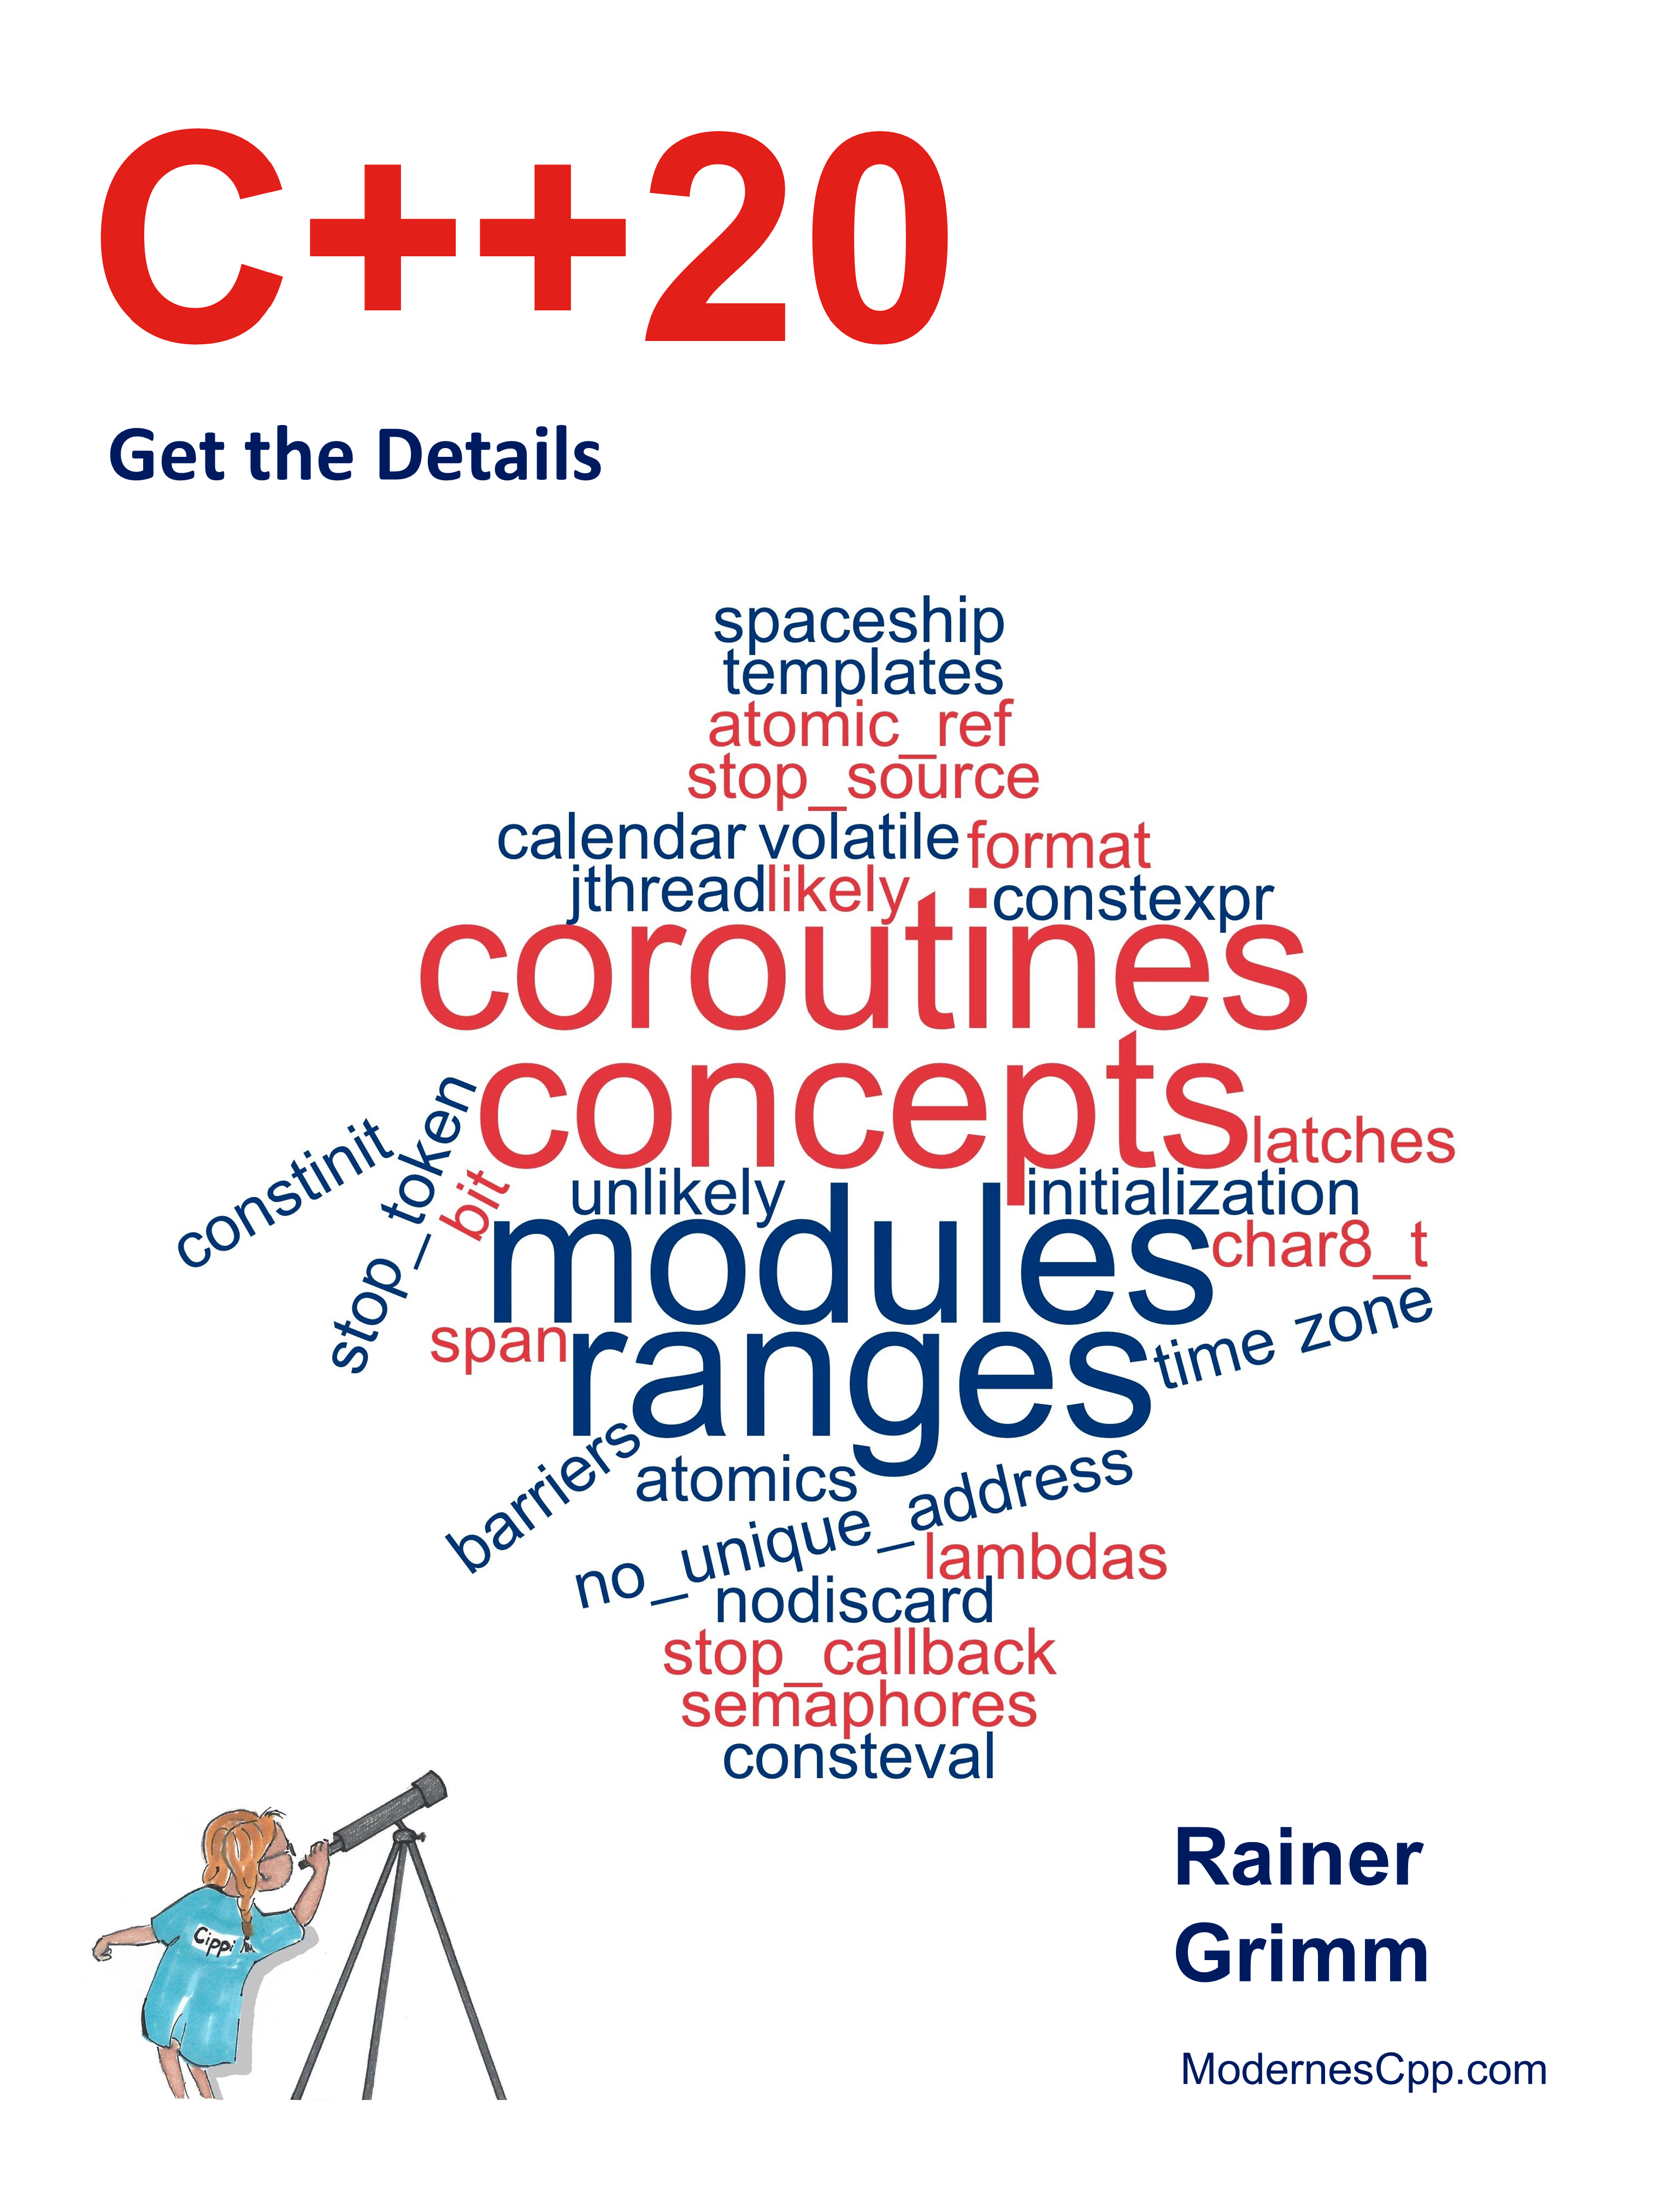
\includegraphics[width=\textwidth,height=\textheight,keepaspectratio]{cover.jpg}
    \begin{tikzpicture}[remember picture, overlay, inner sep=0pt]
      \node at (current page.center) 
      {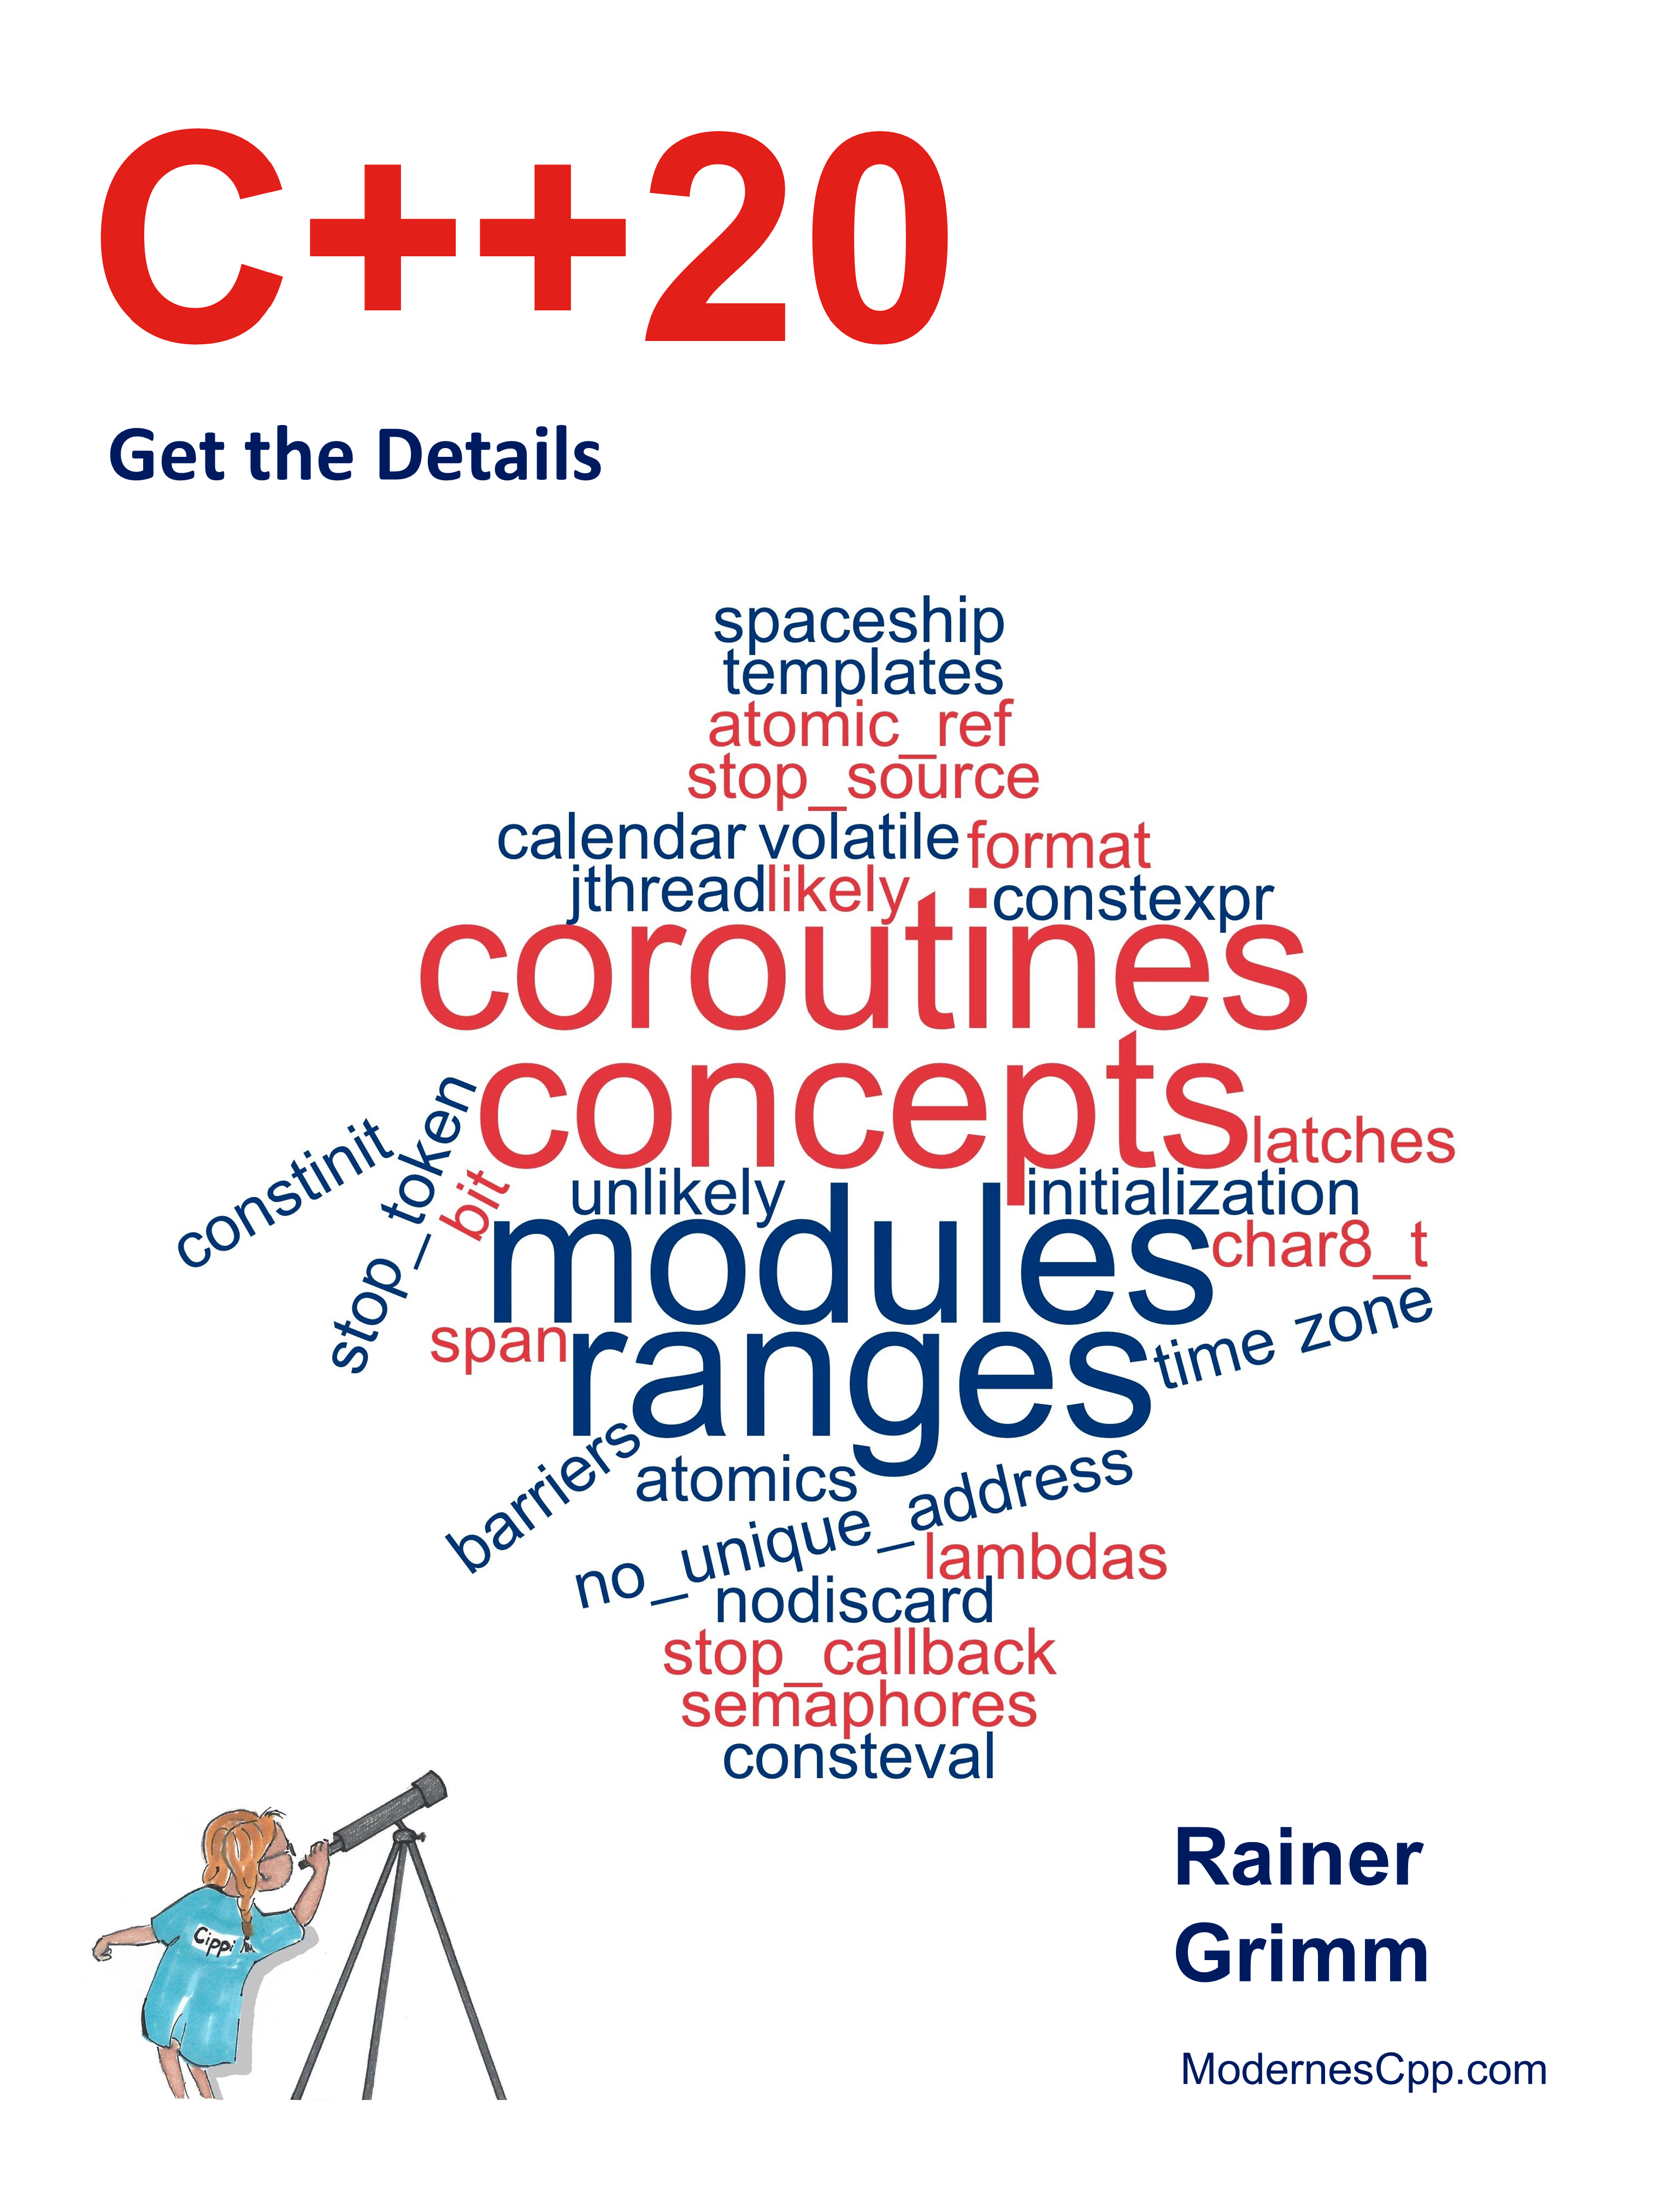
\includegraphics[width=\paperwidth, keepaspectratio=false]{cover.png}};
    \end{tikzpicture}
    \newpage
    \thispagestyle{empty}
    \huge
    \textbf{C++20} 
    \\[9pt]
    \normalsize
    Get the Details
    \\[10pt]
    \normalsize 
    作者: Rainer Grimm 
    \\[8pt]
    \normalsize
    译者:陈晓伟
  \end{center}
  
  \hspace*{\fill} \\ %插入空行
  \noindent\textbf{本书概述}
  
  这本书既是C++20标准的教程,也是参考资料。会教你如何使用C++20,并提供新C++标准的细节。其中,最主要是C++20的四大特性。

  概念(Concept)改变了模板的思考和编程方式,使用模板参数语义,可在类型系统中直接表达可以使用的类型。若出现错误,将出现一条明确的编译错误信息。

  新的“范围”库,能够直接在容器上执行算法,用管道符号组合算法,并可应用到无限数据流上。

  协程(Coroutines)的加入,使得异步编程成为C++的主流。协程是协作任务、事件循环、无限数据流和管道的基础。

  模块(Modules)克服了头文件的限制,例如:头文件和源文件的分离和预处理器一样过时。并且,其可以更快的构建代码和更简单的构建包。

  \hspace*{\fill} \\ %插入空行
  \noindent\textbf{将会了解}
  \begin{itemize}
    \item 自动生成的比较运算符
    \item 日期和时区库
    \item 格式库
    \item 连续的内存块
    \item 加强版可中断线程
    \item 原子智能指针
    \item 信号量
    \item 协调原语,如锁存和栅栏
  \end{itemize}
  
  \hspace*{\fill} \\ %插入空行
  \noindent\textbf{作者简介}
  
  \textbf{Rainer Grimm}自1999年以来一直担任软件架构师、团队领导和讲师。2002年,为公司组织了实习生会议。从2002年起,就开始开设培训课程,第一个教程关于专业管理软件,但不久之后开始教授Python和C++。在业余时间,喜欢写关于C++,Python和Haskell的文章,也喜欢在会议上发言。每周都会在英语博客\href{https://www.modernescpp.com/}{Modernes Cpp}和由\href{https://www.grimm-jaud.de/index.php/blog}{German blog}主办的德语博客上发表文章。
  
  自2016年以来,其一直作为一名独立讲师,在研讨会上讲授现代C++和Python。并用不同的语言出版了几本关于现代C++的书,特别是关于并发性的技术书籍。由于其职业原因,他一直都在寻找教授现代C++的最佳方法。
  
  \hspace*{\fill} \\ %插入空行
  \noindent\textbf{Cippi简介}
  
  来介绍一下Cippi。Cippi将在这本书中陪伴你阅读,希望你能喜欢她。
  
  \begin{center}
  
\includegraphics[width=0.3\textwidth]{content/Cippi.png}\\
  我是Cippi,我好奇、聪明,并且“女人味”十足!!
  \end{center}
  
  Beatrix绘制了Cippi。
  
  \hspace*{\fill} \\ %插入空行
  \noindent\textbf{本书相关}
  \begin{itemize}
  \item Github地址:\url{https://github.com/xiaoweiChen/CXX20-Get-Details}
  \end{itemize}
  \newpage
  
  \pagestyle{empty}
  
  \tableofcontents
  \newpage

  \setsecnumdepth{section}
  
  \color{white}
  \section*{\zihao{1}第一部分:关于C++}
  \pagecolor{mygray}
  \addcontentsline{toc}{section}{第一部分:关于C++}
  \textbf{\subfile{content/1/Section.tex}}
  \newpage
  \color{black}
  \pagecolor{white}

  \subsection*{\zihao{2} 第1章\hspace{0.5cm}历史背景}
  \addcontentsline{toc}{subsection}{第1章\hspace{0.5cm}历史背景}
  \subfile{content/1/chapter1/0.tex}
  
  \subsubsection*{\zihao{3} 1.1.\hspace{0.2cm}C++98}
  \addcontentsline{toc}{subsubsection}{1.1.\hspace{0.2cm}C++98}
  \subfile{content/1/chapter1/1.tex}
  
  \subsubsection*{\zihao{3} 1.2.\hspace{0.2cm}C++03}
  \addcontentsline{toc}{subsubsection}{1.2.\hspace{0.2cm}C++03}
  \subfile{content/1/chapter1/2.tex}
  
  \subsubsection*{\zihao{3} 1.3.\hspace{0.2cm}TR1}
  \addcontentsline{toc}{subsubsection}{1.3.\hspace{0.2cm}TR1}
  \subfile{content/1/chapter1/3.tex}
  
  \subsubsection*{\zihao{3} 1.4.\hspace{0.2cm}C++11}
  \addcontentsline{toc}{subsubsection}{1.4.\hspace{0.2cm}C++11}
  \subfile{content/1/chapter1/4.tex}
  
  \subsubsection*{\zihao{3} 1.5.\hspace{0.2cm}C++14}
  \addcontentsline{toc}{subsubsection}{1.5.\hspace{0.2cm}C++14}
  \subfile{content/1/chapter1/5.tex}
  
  \subsubsection*{\zihao{3} 1.6.\hspace{0.2cm}C++17}
  \addcontentsline{toc}{subsubsection}{1.6.\hspace{0.2cm}C++17}
  \subfile{content/1/chapter1/6.tex}
  \newpage
  
  \subsection*{\zihao{2} 第2章\hspace{0.5cm}标准化}
  \addcontentsline{toc}{subsection}{第2章\hspace{0.5cm}标准化}
  \subfile{content/1/chapter2/0.tex}
  
  \subsubsection*{\zihao{3} 2.1.\hspace{0.2cm}阶段 3}
  \addcontentsline{toc}{subsubsection}{2.1.\hspace{0.2cm}阶段 3}
  \subfile{content/1/chapter2/1.tex}
  
  \subsubsection*{\zihao{3} 2.2.\hspace{0.2cm}阶段 2}
  \addcontentsline{toc}{subsubsection}{2.2.\hspace{0.2cm}阶段 2}
  \subfile{content/1/chapter2/2.tex}
  
  \subsubsection*{\zihao{3} 2.3.\hspace{0.2cm}阶段 1}
  \addcontentsline{toc}{subsubsection}{2.3.\hspace{0.2cm}阶段 1}
  \subfile{content/1/chapter2/3.tex}
  \newpage
  
  \color{white}
  \section*{\zihao{1}第二部分:概述C++20}
  \pagecolor{mygray}
  \addcontentsline{toc}{section}{第二部分:概述C++20}
  \textbf{\subfile{content/2/Section.tex}}
  \newpage
  \color{black}
  \pagecolor{white}
  
  \subsection*{\zihao{2} 第3章\hspace{0.5cm}C++20}
  \addcontentsline{toc}{subsection}{第3章\hspace{0.5cm}C++20}
  \subfile{content/2/chapter3/0.tex}
  
  \subsubsection*{\zihao{3} 3.1.\hspace{0.2cm}四大新特性}
  \addcontentsline{toc}{subsubsection}{3.1.\hspace{0.2cm}四大新特性}
  \subfile{content/2/chapter3/1.tex}
  
  \subsubsection*{\zihao{3} 3.2.\hspace{0.2cm}核心语言特性}
  \addcontentsline{toc}{subsubsection}{3.2.\hspace{0.2cm}核心语言特性}
  \subfile{content/2/chapter3/2.tex}
  
  \subsubsection*{\zihao{3} 3.3.\hspace{0.2cm}标准库}
  \addcontentsline{toc}{subsubsection}{3.3.\hspace{0.2cm}标准库}
  \subfile{content/2/chapter3/3.tex}
  
  \subsubsection*{\zihao{3} 3.4.\hspace{0.2cm}并发性}
  \addcontentsline{toc}{subsubsection}{3.4.\hspace{0.2cm}并发性}
  \subfile{content/2/chapter3/4.tex}
  \newpage
  
  \color{white}
  \section*{\zihao{1}第三部分:特性详情}
  \pagecolor{mygray}
  \addcontentsline{toc}{section}{第三部分:特性详情}
  \textbf{\subfile{content/3/Section.tex}}
  \newpage
  \color{black}
  \pagecolor{white}
  
  \subsection*{\zihao{2} 第4章\hspace{0.5cm}语言核心}
  \addcontentsline{toc}{subsection}{第4章\hspace{0.5cm}语言核心}
  \subfile{content/3/chapter4/0.tex}
  
  \subsubsection*{\zihao{3} 4.1.\hspace{0.2cm}概念}
  \addcontentsline{toc}{subsubsection}{4.1.\hspace{0.2cm}概念}
  \subfile{content/3/chapter4/1.tex}
  
  \subsubsection*{\zihao{3} 4.2.\hspace{0.2cm}模块}
  \addcontentsline{toc}{subsubsection}{4.2.\hspace{0.2cm}模块}
  \subfile{content/3/chapter4/2.tex}
  
  \subsubsection*{\zihao{3} 4.3.\hspace{0.2cm}三向比较操作符}
  \addcontentsline{toc}{subsubsection}{4.3.\hspace{0.2cm}三向比较操作符}
  \subfile{content/3/chapter4/3.tex}
  
  \subsubsection*{\zihao{3} 4.4.\hspace{0.2cm}指定初始化}
  \addcontentsline{toc}{subsubsection}{4.4.\hspace{0.2cm}指定初始化}
  \subfile{content/3/chapter4/4.tex}
  
  \subsubsection*{\zihao{3} 4.5.\hspace{0.2cm}consteval和constinit}
  \addcontentsline{toc}{subsubsection}{4.5.\hspace{0.2cm}consteval和constinit}
  \subfile{content/3/chapter4/5.tex}
  
  \subsubsection*{\zihao{3} 4.6.\hspace{0.2cm}模板的改进}
  \addcontentsline{toc}{subsubsection}{4.6.\hspace{0.2cm}模板的改进}
  \subfile{content/3/chapter4/6.tex}
  
  \subsubsection*{\zihao{3} 4.7.\hspace{0.2cm}Lambda的改进}
  \addcontentsline{toc}{subsubsection}{4.7.\hspace{0.2cm}Lambda的改进}
  \subfile{content/3/chapter4/7.tex}
  
  \subsubsection*{\zihao{3} 4.8.\hspace{0.2cm}新属性}
  \addcontentsline{toc}{subsubsection}{4.8.\hspace{0.2cm}新属性}
  \subfile{content/3/chapter4/8.tex}
  
  \subsubsection*{\zihao{3} 4.9.\hspace{0.2cm}进一步的改善}
  \addcontentsline{toc}{subsubsection}{4.9.\hspace{0.2cm}进一步的改善}
  \subfile{content/3/chapter4/9.tex}
  \newpage

  \subsection*{\zihao{2} 第5章\hspace{0.5cm}标准库}
  \addcontentsline{toc}{subsection}{第5章\hspace{0.5cm}标准库}
  \subfile{content/3/chapter5/0.tex}
  
  \subsubsection*{\zihao{3} 5.1.\hspace{0.2cm}范围库}
  \addcontentsline{toc}{subsubsection}{5.1.\hspace{0.2cm}范围库}
  \subfile{content/3/chapter5/1.tex}
  
  \subsubsection*{\zihao{3} 5.2.\hspace{0.2cm}std::span}
  \addcontentsline{toc}{subsubsection}{5.2.\hspace{0.2cm}std::span}
  \subfile{content/3/chapter5/2.tex}
  
  \subsubsection*{\zihao{3} 5.3.\hspace{0.2cm}容器的改进}
  \addcontentsline{toc}{subsubsection}{5.3.\hspace{0.2cm}容器的改进}
  \subfile{content/3/chapter5/3.tex}
  
  \subsubsection*{\zihao{3} 5.4.\hspace{0.2cm}算术工具}
  \addcontentsline{toc}{subsubsection}{5.4.\hspace{0.2cm}算术工具}
  \subfile{content/3/chapter5/4.tex}
  
  \subsubsection*{\zihao{3} 5.5.\hspace{0.2cm}日期和时区}
  \addcontentsline{toc}{subsubsection}{5.5.\hspace{0.2cm}日期和时区}
  \subfile{content/3/chapter5/5.tex}
  
  \subsubsection*{\zihao{3} 5.6.\hspace{0.2cm}格式库}
  \addcontentsline{toc}{subsubsection}{5.6.\hspace{0.2cm}格式库}
  \subfile{content/3/chapter5/6.tex}
  
  \subsubsection*{\zihao{3} 5.7.\hspace{0.2cm}进一步的改善}
  \addcontentsline{toc}{subsubsection}{5.7.\hspace{0.2cm}进一步的改善}
  \subfile{content/3/chapter5/7.tex}
  \newpage
  
  \subsection*{\zihao{2} 第6章\hspace{0.5cm}并发性}
  \addcontentsline{toc}{subsection}{第6章\hspace{0.5cm}并发性}
  \subfile{content/3/chapter6/0.tex}
  
  \subsubsection*{\zihao{3} 6.1.\hspace{0.2cm}协程}
  \addcontentsline{toc}{subsubsection}{6.1.\hspace{0.2cm}协程}
  \subfile{content/3/chapter6/1.tex}
  
  \subsubsection*{\zihao{3} 6.2.\hspace{0.2cm}原子}
  \addcontentsline{toc}{subsubsection}{6.2.\hspace{0.2cm}原子}
  \subfile{content/3/chapter6/2.tex}
  
  \subsubsection*{\zihao{3} 6.3.\hspace{0.2cm}信号量}
  \addcontentsline{toc}{subsubsection}{6.3.\hspace{0.2cm}信号量}
  \subfile{content/3/chapter6/3.tex}
  
  \subsubsection*{\zihao{3} 6.4.\hspace{0.2cm}门闩和栅栏}
  \addcontentsline{toc}{subsubsection}{6.4.\hspace{0.2cm}门闩和栅栏}
  \subfile{content/3/chapter6/4.tex}
  
  \subsubsection*{\zihao{3} 6.5.\hspace{0.2cm}中断协程}
  \addcontentsline{toc}{subsubsection}{6.5.\hspace{0.2cm}中断协程}
  \subfile{content/3/chapter6/5.tex}
  
  \subsubsection*{\zihao{3} 6.6.\hspace{0.2cm}std::jthread}
  \addcontentsline{toc}{subsubsection}{6.6.\hspace{0.2cm}std::jthread}
  \subfile{content/3/chapter6/6.tex}
  
  \subsubsection*{\zihao{3} 6.7.\hspace{0.2cm}同步输出流}
  \addcontentsline{toc}{subsubsection}{6.7.\hspace{0.2cm}同步输出流}
  \subfile{content/3/chapter6/7.tex}
  \newpage
  
  \subsection*{\zihao{2} 第7章\hspace{0.5cm}相关案例}
  \addcontentsline{toc}{subsection}{第7章\hspace{0.5cm}相关案例}
  \subfile{content/3/chapter7/0.tex}
  
  \subsubsection*{\zihao{3} 7.1.\hspace{0.2cm}线程的快速同步}
  \addcontentsline{toc}{subsubsection}{7.1.\hspace{0.2cm}线程的快速同步}
  \subfile{content/3/chapter7/1.tex}
  
  \subsubsection*{\zihao{3} 7.2.\hspace{0.2cm}Future的变体}
  \addcontentsline{toc}{subsubsection}{7.2.\hspace{0.2cm}Future的变体}
  \subfile{content/3/chapter7/2.tex}
  
  \subsubsection*{\zihao{3} 7.3.\hspace{0.2cm}生成器的修改和泛化}
  \addcontentsline{toc}{subsubsection}{7.3.\hspace{0.2cm}生成器的修改和泛化}
  \subfile{content/3/chapter7/3.tex}
  
  \subsubsection*{\zihao{3} 7.4.\hspace{0.2cm}不同的工作流}
  \addcontentsline{toc}{subsubsection}{7.4.\hspace{0.2cm}不同的工作流}
  \subfile{content/3/chapter7/4.tex}
  \newpage
  
  \color{white}
  \section*{\zihao{1}第四部分:后记}
  \pagecolor{mygray}
  \addcontentsline{toc}{section}{第四部分:后记}
  \textbf{\subfile{content/4/Section.tex}}
  \newpage
  \color{black}
  \pagecolor{white}
  \newpage
  
  \color{white}
  \section*{\zihao{1}第五部分:更多信息}
  \pagecolor{mygray}
  \addcontentsline{toc}{section}{第五部分:更多信息}
  \textbf{\subfile{content/5/Section.tex}}
  \newpage
  \color{black}
  \pagecolor{white}
  \newpage
  
  \subsection*{\zihao{2} 第8章\hspace{0.5cm}C++23和之后的标准}
  \addcontentsline{toc}{subsection}{第8章\hspace{0.5cm}C++23和之后的标准}
  \subfile{content/5/chapter8/0.tex}
  
  \subsubsection*{\zihao{3} 8.1.\hspace{0.2cm}C++23}
  \addcontentsline{toc}{subsubsection}{8.1.\hspace{0.2cm}C++23}
  \subfile{content/5/chapter8/1.tex}
  
  \subsubsection*{\zihao{3} 8.2.\hspace{0.2cm}C++23或之后的标准}
  \addcontentsline{toc}{subsubsection}{8.2.\hspace{0.2cm}C++23或之后的标准}
  \subfile{content/5/chapter8/2.tex}
  
  \subsubsection*{\zihao{3} 8.3.\hspace{0.2cm}C++23的更多信息}
  \addcontentsline{toc}{subsubsection}{8.3.\hspace{0.2cm}C++23的更多信息}
  \subfile{content/5/chapter8/3.tex}
  \newpage
  
  \subsection*{\zihao{2} 第9章\hspace{0.5cm}功能测试}
  \addcontentsline{toc}{subsection}{第9章\hspace{0.5cm}功能测试}
  \subfile{content/5/chapter9/0.tex}
  \newpage
  
  \subsection*{\zihao{2} 第10章\hspace{0.5cm}术语表}
  \addcontentsline{toc}{subsection}{第10章\hspace{0.5cm}术语表}
  \subfile{content/5/chapter10/0.tex}
  
  \subsubsection*{\zihao{3} 10.1.\hspace{0.2cm}可调用}
  \addcontentsline{toc}{subsubsection}{10.1.\hspace{0.2cm}可调用}
  \subfile{content/5/chapter10/1.tex}
  
  \subsubsection*{\zihao{3} 10.2.\hspace{0.2cm}可调用单元}
  \addcontentsline{toc}{subsubsection}{10.2.\hspace{0.2cm}可调用单元}
  \subfile{content/5/chapter10/2.tex}
  
  \subsubsection*{\zihao{3} 10.3.\hspace{0.2cm}并发性}
  \addcontentsline{toc}{subsubsection}{10.3.\hspace{0.2cm}并发性}
  \subfile{content/5/chapter10/3.tex}
  
  \subsubsection*{\zihao{3} 10.4.\hspace{0.2cm}临界区}
  \addcontentsline{toc}{subsubsection}{10.4.\hspace{0.2cm}临界区}
  \subfile{content/5/chapter10/4.tex}
  
  \subsubsection*{\zihao{3} 10.5.\hspace{0.2cm}数据竞争}
  \addcontentsline{toc}{subsubsection}{10.5.\hspace{0.2cm}数据竞争}
  \subfile{content/5/chapter10/5.tex}
  
  \subsubsection*{\zihao{3} 10.6.\hspace{0.2cm}死锁}
  \addcontentsline{toc}{subsubsection}{10.6.\hspace{0.2cm}死锁}
  \subfile{content/5/chapter10/6.tex}
  
  \subsubsection*{\zihao{3} 10.7.\hspace{0.2cm}立即求值}
  \addcontentsline{toc}{subsubsection}{10.7.\hspace{0.2cm}立即求值}
  \subfile{content/5/chapter10/7.tex}
  
  \subsubsection*{\zihao{3} 10.8.\hspace{0.2cm}
  	执行器}
  \addcontentsline{toc}{subsubsection}{10.8.\hspace{0.2cm}执行器}
  \subfile{content/5/chapter10/8.tex}
  
  \subsubsection*{\zihao{3} 10.9.\hspace{0.2cm}函数对象}
  \addcontentsline{toc}{subsubsection}{10.9.\hspace{0.2cm}函数对象}
  \subfile{content/5/chapter10/9.tex}
  
  \subsubsection*{\zihao{3} 10.10.\hspace{0.2cm}Lambda表达式}
  \addcontentsline{toc}{subsubsection}{10.10.\hspace{0.2cm}Lambda表达式}
  \subfile{content/5/chapter10/10.tex}
  
  \subsubsection*{\zihao{3} 10.11.\hspace{0.2cm}延迟(惰性)求值}
  \addcontentsline{toc}{subsubsection}{10.11.\hspace{0.2cm}延迟(惰性)求值}
  \subfile{content/5/chapter10/11.tex}
  
  \subsubsection*{\zihao{3} 10.12.\hspace{0.2cm}无锁}
  \addcontentsline{toc}{subsubsection}{10.12.\hspace{0.2cm}无锁}
  \subfile{content/5/chapter10/12.tex}
  
  \subsubsection*{\zihao{3} 10.13.\hspace{0.2cm}错过唤醒}
  \addcontentsline{toc}{subsubsection}{10.13.\hspace{0.2cm}错过唤醒}
  \subfile{content/5/chapter10/13.tex}
  
  \subsubsection*{\zihao{3} 10.14.\hspace{0.2cm}数学规律}
  \addcontentsline{toc}{subsubsection}{10.14.\hspace{0.2cm}数学规律}
  \subfile{content/5/chapter10/14.tex}
  
  \subsubsection*{\zihao{3} 10.15.\hspace{0.2cm}内存位置}
  \addcontentsline{toc}{subsubsection}{10.15.\hspace{0.2cm}内存位置}
  \subfile{content/5/chapter10/15.tex}
  
  \subsubsection*{\zihao{3} 10.16.\hspace{0.2cm}内存模型}
  \addcontentsline{toc}{subsubsection}{10.16.\hspace{0.2cm}内存模型}
  \subfile{content/5/chapter10/16.tex}
  
  \subsubsection*{\zihao{3} 10.17.\hspace{0.2cm}非阻塞}
  \addcontentsline{toc}{subsubsection}{10.17.\hspace{0.2cm}非阻塞}
  \subfile{content/5/chapter10/17.tex}
  
  \subsubsection*{\zihao{3} 10.18.\hspace{0.2cm}对象}
  \addcontentsline{toc}{subsubsection}{10.18.\hspace{0.2cm}对象}
  \subfile{content/5/chapter10/18.tex}
  
  \subsubsection*{\zihao{3} 10.19.\hspace{0.2cm}并行性}
  \addcontentsline{toc}{subsubsection}{10.19.\hspace{0.2cm}并行性}
  \subfile{content/5/chapter10/19.tex}
  
  \subsubsection*{\zihao{3} 10.20.\hspace{0.2cm}谓词}
  \addcontentsline{toc}{subsubsection}{10.20.\hspace{0.2cm}谓词}
  \subfile{content/5/chapter10/20.tex}
  
  \subsubsection*{\zihao{3} 10.21.\hspace{0.2cm}RAII(资源获取即初始化)}
  \addcontentsline{toc}{subsubsection}{10.21.\hspace{0.2cm}RAII(资源获取即初始化)}
  \subfile{content/5/chapter10/21.tex}
  
  \subsubsection*{\zihao{3} 10.22.\hspace{0.2cm}竞态条件}
  \addcontentsline{toc}{subsubsection}{10.22.\hspace{0.2cm}竞态条件}
  \subfile{content/5/chapter10/22.tex}
  
  \subsubsection*{\zihao{3} 10.23.\hspace{0.2cm}常规类型}
  \addcontentsline{toc}{subsubsection}{10.23.\hspace{0.2cm}常规类型}
  \subfile{content/5/chapter10/23.tex}
  
  \subsubsection*{\zihao{3} 10.24.\hspace{0.2cm}标量}
  \addcontentsline{toc}{subsubsection}{10.24.\hspace{0.2cm}标量}
  \subfile{content/5/chapter10/24.tex}
  
  \subsubsection*{\zihao{3} 10.25.\hspace{0.2cm}半常规类型}
  \addcontentsline{toc}{subsubsection}{10.25.\hspace{0.2cm}半常规类型}
  \subfile{content/5/chapter10/25.tex}
  
  \subsubsection*{\zihao{3} 10.26.\hspace{0.2cm}伪唤醒}
  \addcontentsline{toc}{subsubsection}{10.26.\hspace{0.2cm}伪唤醒}
  \subfile{content/5/chapter10/26.tex}
  
  \subsubsection*{\zihao{3} 10.27.\hspace{0.2cm}四大特性}
  \addcontentsline{toc}{subsubsection}{10.27.\hspace{0.2cm}四大特性}
  \subfile{content/5/chapter10/27.tex}
  
  \subsubsection*{\zihao{3} 10.28.\hspace{0.2cm}六大函数}
  \addcontentsline{toc}{subsubsection}{10.28.\hspace{0.2cm}六大函数}
  \subfile{content/5/chapter10/28.tex}
  
  \subsubsection*{\zihao{3} 10.29.\hspace{0.2cm}线程}
  \addcontentsline{toc}{subsubsection}{10.29.\hspace{0.2cm}线程}
  \subfile{content/5/chapter10/29.tex}
  
  \subsubsection*{\zihao{3} 10.30.\hspace{0.2cm}时间复杂度}
  \addcontentsline{toc}{subsubsection}{10.30.\hspace{0.2cm}时间复杂度}
  \subfile{content/5/chapter10/30.tex}
  
  \subsubsection*{\zihao{3} 10.31.\hspace{0.2cm}翻译单元}
  \addcontentsline{toc}{subsubsection}{10.31.\hspace{0.2cm}翻译单元}
  \subfile{content/5/chapter10/31.tex}
  
  \subsubsection*{\zihao{3} 10.32.\hspace{0.2cm}未定义行为}
  \addcontentsline{toc}{subsubsection}{10.32.\hspace{0.2cm}未定义行为}
  \subfile{content/5/chapter10/32.tex}
  \newpage

\end{sloppypar}
\end{document}

